%%% for platex
\documentclass[a4paper,12pt,dvipdfmx]{jbook}
%%% for lualatex
%\documentclass[a4paper,12pt]{ltjbook}

\usepackage{master}
%%%%%%%%%%%%%%%%%%%%%%%%%%%%%%%%%%%%%%%%%%%%%%%%%%%%%%%%%%%%%%%%
% User-defined Macro
%%%%%%%%%%%%%%%%%%%%%%%%%%%%%%%%%%%%%%%%%%%%%%%%%%%%%%%%%%%%%%%%
\newcommand{\compress}{\itemsep0pt\parsep0pt\parskip0pt\partopsep0pt}
% \newcommand{\compress}{\itemsep1pt plus1pt\parsep0pt\parskip0pt}
% \newcommand{\code}[1]{\lstinline[basicstyle=\ttfamily]{#1}}
\newcommand{\gringo}{\textit{gringo}}
\newcommand{\clasp}{\textit{clasp}}
\newcommand{\clingo}{\textit{clingo}}
\newcommand{\teaspoon}{\textit{teaspoon}}
\newcommand{\sat}{\textsf{SAT}}
\newcommand{\unsat}{\textsf{UNSAT}}
% \newcommand{\web}[2]{\href{#1}{#2\ \raisebox{-0.15ex}{\beamergotobutton{Web}}}}
% \newcommand{\doi}[2]{\href{#1}{#2\ \raisebox{-0.15ex}{\beamergotobutton{DOI}}}}
% \newcommand{\weblink}[1]{\web{#1}{#1}}
% \newcommand{\imp}{\mathrel{\Rightarrow}}
% \newcommand{\Iff}{\mathrel{\Leftrightarrow}}
% \newcommand{\mybox}[1]{\fbox{\rule[.2cm]{0cm}{0cm}\mbox{${#1}$}}}
% \newcommand{\mycbox}[2]{\tikz[baseline]\node[fill=#1!10,anchor=base,rounded corners=2pt] () {#2};}
% \newcommand{\naf}[1]{\ensuremath{{\sim\!\!{#1}}}}
% \newcommand{\head}[1]{\ensuremath{\mathit{head}(#1)}}
% \newcommand{\body}[1]{\ensuremath{\mathit{body}(#1)}}
% \newcommand{\atom}[1]{\ensuremath{\mathit{atom}(#1)}}
% \newcommand{\poslits}[1]{\ensuremath{{#1}^+}}
% \newcommand{\neglits}[1]{\ensuremath{{#1}^-}}
% \newcommand{\pbody}[1]{\poslits{\body{#1}}}
% \newcommand{\nbody}[1]{\neglits{\body{#1}}}
% \newcommand{\Cn}[1]{\ensuremath{\mathit{Cn}(#1)}}
% \newcommand{\reduct}[2]{\ensuremath{#1^{#2}}}
% \newcommand{\OK}{\mbox{\textcolor{green}{\Pisymbol{pzd}{52}}}}
% \newcommand{\KO}{\mbox{\textcolor{red}{\Pisymbol{pzd}{56}}}}
% \newcommand{\code}[1]{\lstinline[basicstyle=\ttfamily]{#1}}
% \newcommand{\lw}[1]{\smash{\lower2.ex\hbox{#1}}}
\newcommand{\llw}[1]{\smash{\lower3.ex\hbox{#1}}}

\newenvironment{tableC}{%
  \scriptsize
  \renewcommand{\arraystretch}{0.9}
  \tabcolsep = 0.6mm
  % \begin{tabular}[t]{p{6mm}|rlr|rlr|rlr|rlr|rlr}\hline
  %   \multicolumn{1}{l|}{\llw{問題   }} &
  \begin{tabular}[t]{l|rlr|rlr|rlr|rlr|rlr}\hline
    \multicolumn{1}{l|}{\llw{問題}} &
    \multicolumn{3}{c|}{UD1} &
    \multicolumn{3}{c|}{UD2} &
    \multicolumn{3}{c|}{UD3} &
    \multicolumn{3}{c|}{UD4} &
    \multicolumn{3}{c}{UD5} \\
    & 
    \multicolumn{1}{c}{既知の} & & \multicolumn{1}{c|}{ASP} & 
    \multicolumn{1}{c}{既知の} & & \multicolumn{1}{c|}{ASP} & 
    \multicolumn{1}{c}{既知の} & & \multicolumn{1}{c|}{ASP} & 
    \multicolumn{1}{c}{既知の} & & \multicolumn{1}{c|}{ASP} & 
    \multicolumn{1}{c}{既知の} & & \multicolumn{1}{c}{ASP} \\
    & 
    ベスト & &  & 
    ベスト & &  & 
    ベスト & &  & 
    ベスト & &  & 
    ベスト & &  \\
    \hline
  }{%
    \hline
  \end{tabular}
}
 % 自分用のマクロ

%%%%%%%%%%%%%%%%%%%%%%%%%%%%%%%%%%%%%%%%%%%%%%%%%%%%%%%%%%
% タイトル
%%%%%%%%%%%%%%%%%%%%%%%%%%%%%%%%%%%%%%%%%%%%%%%%%%%%%%%%%%
\bookname{修 士 論 文}
\institute{名古屋大学大学院情報学研究科}
\major{情報システム学専攻}
\title{解集合プログラミングに基づく\\
系統的探索と確率的局所探索の\\
統合的手法に関する研究}
\date{2021年度}
\author{桑原 和也}
\studentid{252005066}

%%%%%%%%%%%%%%%%%%%%%%%%%%%%%%%%%%%%%%%%%%%%%%%%%%%%%%%%%% 
% 本体
%%%%%%%%%%%%%%%%%%%%%%%%%%%%%%%%%%%%%%%%%%%%%%%%%%%%%%%%%% 
\begin{document}
\maketitle

%%%%%%%%%%%%%%%%%%%%%%%%%%%%%%%%%%%%%%%%%%%%%%%%%%%%%%%%%% 
\chapter*{概要}
\pagenumbering{roman}
%%%%%%%%%%%%%%%%%%%%%%%%%%%%%%%%%%%%%%%%%%%%%%%%%%%%%%%%%% 

本論文では,解集合プログラミングを用いた組合せ遷移問題の解法について述べる.
組合せ遷移問題とは,ある組合せ問題とその2つの実行可能解が与えられたとき,
一方の実行可能解から他方の実行可能解へ,
遷移制約を満たしつつ到達できるかを判定する問題である.

$k$彩色遷移問題は組合せ遷移問題の一つであり,
色数$k$のグラフ点彩色問題と二つの彩色が与えられたとき,
一方の彩色から他方の彩色へ,各遷移過程において色が変化する頂点はただ一つ
という遷移制約を満たしつつ,到達できるかを判定する問題である.
一般に,$k \ge 4$において PSPACE 完全であることが知られている.

解集合プログラミング(ASP)は,論理プログラムから派生したプログラミングパラダイムである.
ASP 言語は一階論理に基づいた知識表現言語の一種である.
論理プログラムはルールの有限集合である.
ASP システムは解集合を計算するシステムである.

本論文では,解集合プログラミング(ASP)を用いた$k$彩色遷移問題の解法について述べる.
本研究では問題の入力に遷移回数$t$を加え,「遷移回数$t$での経路の存在」を解く.
まず,$k$彩色遷移問題を解く3種類の ASP 符号化,
\code{vrc1},\code{vrc2},\code{vrc3}を提案した.
特に\code{vrc3}では基礎化後のルール数を少なく抑えているため,
大規模な問題に対する有効性が期待できる.

提案した符号化を評価するにあたり,
独自に生成した90問のベンチマークを使用し評価実験を行った.
その結果,すべての符号化で90問中11問で到達可能であることを判定できた.
さらに,\textsf{vrc3}符号化は,多くの問題で判定に要した CPU 時間が短く,
その優位性が確認できた.

%%% Local Variables:
%%% mode: japanese-latex
%%% TeX-master: "paper"
%%% End:    % 概要

\tableofcontents    % 目次
\listoffigures      % 図の目次
\listoftables       % 表の目次
\lstlistoflistings  % コードの目次

% ここから「本文」
%%%%%%%%%%%%%%%%%%%%%%%%%%%%%%%%%%%%%%%%%%%%%%%%%%%%%%%%%% 
\chapter{序論}
\pagenumbering{arabic}
%%%%%%%%%%%%%%%%%%%%%%%%%%%%%%%%%%%%%%%%%%%%%%%%%%%%%%%%%% 

\textbf{ハミルトン閉路問題 (Hamiltonian Cycle Problem)} は,
与えられたグラフの全頂点をちょうど一度ずつ通る閉路が存在するかどうかを
判定する問題である.
\textbf{ハミルトン路問題 (Hamiltonian Path Problem)} は,
ハミルトン閉路問題から始点と終点が一致するという閉路の条件を取り除いた
ものである.
ハミルトン閉路問題とハミルトン路問題は,どちらも NP 完全な問題である.
これらの問題は,重要な工学的応用が数多く存在するため,古くから盛んに研
究されている.
例えば,数理最適化の分野で有名な巡回セールスマン問題は,グラフの辺に距
離が付随しているとき,最短距離のハミルトン閉路を求める
\textbf{最短ハミルトン閉路問題}と考えることができる.
また,ごく最近では,距離の総和が所与の閾値以下(または以上)であることを
制約条件として付加した
\textbf{コスト制約付きハミルトン閉路問題}\cite{comp20:Minato}
も提案されている.
本研究では,無向グラフ上のハミルトン閉路問題およびその関連問題を対象とする.

解集合プログラミング(Answer Set Programming; ASP)は,
論理プログラミングから派生した比較的新しいプログラミングパラダイムである.
ASP言語は,一階論理に基づく知識表現言語の一種であり,
論理プログラムは ASP のルールの有限集合である.
ASP システムは論理プログラムから安定モデル意味論に基づく解集合を計算す
るシステムである.
近年,SAT技術を応用した高速 ASP システムが開発され,スケジューリング,
プランニング,システム生物学,システム検証,制約充足問題,
制約最適化問題など様々な分野への実用的応用が急速に拡大している.
ハミルトン閉路問題およびその関連問題に対して ASP を用いる利点としては,
ASP 言語の高い表現力,
充足不能コアに基づく最適化,
インクリメンタルASP解法,
組込み非閉路制約,
高速な解列挙
などが挙げられる.

本論文では,解集合プログラミング(ASP)を用いた
ハミルトン閉路問題,
最短ハミルトン閉路問題,
コスト制約付きハミルトン閉路問題
の解法について述べる.
%
ハミルトン閉路問題を解くASP符号化として,
\textsf{undirected},
\textsf{directed},
\textsf{acyclicity}
の3つを考案した.
\textsf{undirected}は,
ハミルトン閉路問題を次数制約と部分閉路禁止制約で簡潔に表現した符号化である.
\textsf{directed}は,
与えられた無向グラフの各辺$u-v$に対して,
2つの弧$u\rightarrow v$と$v\rightarrow u$を対応させることで有向グラフ
化して解く符号化である.
変換した有向グラフ上のハミルトン閉路は元の無向グラフ上のハミルトン閉路
となり,また逆も成り立つ.
\textsf{acyclicity}は,\textsf{directed}符号化をベースに,
部分閉路禁止制約を組込み非閉路制約で表現した符号化である.
\textsf{acyclicity}符号化は,他の二つと比較して,基礎化後の制約数を少
なく抑えることができるため,大規模な問題に対する有効性が期待できる.
最短ハミルトン閉路問題とコスト制約付きハミルトン閉路問題については,
考案した3つの符号化に目的関数とコスト制約をそれぞれ追加することで自然に拡張できる.

考案した符号化の有効性を評価するために,
既存のベンチマーク問題集(7種類,計516問)を用いて実行実験を行なった.
その結果,
ハミルトン閉路問題とコスト制約付きハミルトン閉路問題(解の全列挙)について,
\textsf{acyclicity}符号化が,
\textsf{undirected}と\textsf{directed}と比較して,
より多くの問題を高速に解くことに成功し,その優位性を確認できた.
また,最短ハミルトン閉路問題については,
\textsf{undirected}符号化が,他の符号化と比較して,より多くの問題で最
適値・最良値を求めることができた.

%%% Local Variables:
%%% mode: latex
%%% TeX-master: "paper"
%%% End:

\section{解集合プログラミング} \label{chap:asp}

\textbf{解集合プログラミング} (Answer Set Programming; ASP~\cite{%
  Baral03:cambridge,%
  Gelfond88:iclp,%
  Inoue08:jssst,%
  Niemela99:amai})
は,演繹データベース,否定を含む論理プログラミング,
非単調推論,制約充足 (特に,SAT)を起源にもつ,
宣言的プログラミングパラダイムである.
ASP の言語は,一般拡張選言プログラムに基づいている.
本稿では説明の簡略化のため,そのサブクラスである
標準論理プログラムについて説明する.
以降,標準論理プログラムを単に論理プログラムとよぶ.

\textbf{論理プログラム}は,以下の形式をした\textbf{ルール}の有限集合である.
\[
  a_0\leftarrow a_1,\dots,a_m,\naf{a_{m+1}},\dots,\naf{a_n}
\]
ここで,
$0\leq m\leq n$ であり,
各$a_i$はアトム,
$\naf{}$はデフォルトの否定
\footnote{``失敗による否定''ともよばれる.述語論理で定義される否定($\neg$)とは意味が異なる.},
``$,$''は連言を表す.
$\leftarrow$の左側をヘッド,右側をボディとよぶ.
ルールの直観的な意味は,
「$a_1,\ldots,a_m$がすべて成り立ち,$a_{m+1},\ldots,a_n$のそれぞれが成
り立たないならば,$a_0$が成り立つ」である.
ボディが空のルール(すなわち\(a_0\leftarrow\))を\textbf{ファクト}とよび,
$\leftarrow$を省略してよい.

ヘッドが空のルールを\textbf{一貫性制約}とよぶ.
\[
  \leftarrow a_1,\dots,a_m,\naf{a_{m+1}},\dots,\naf{a_n}
\]

直観的には,\(\leftarrow a_1\)は,「$a_1$ではない」という禁止を表し,
\(\leftarrow \naf{a_1}\)は,「$a_1$でなければならない」という強制を表す.
また,
%\(\leftarrow a_1,a_2\)は,「$a_1$と$a_2$が両方同時に成り立つことはない」を意味し,
\(\leftarrow a_1, \naf{a_{2}}\)は,「$a_1$が成り立つならば,$a_2$が成り立つ」を意味する.

ASP 言語は,組合せ問題を解くための便利な拡張構文を備えている.
その代表的なものが\textbf{選択子}と\textbf{個数制約}である.
例えば,選択子\(\{a_1;\dots;a_n\}\)をファクトとして書くと,
「アトム集合\(\{a_1,\dots,a_n\}\)の任意の部分集合が成り立つ」を意味する.
個数制約は選択子の両端に選択可能な個数の上下限を付けたものである.
例えば,\(lb\ \{a_1;\dots;a_n\}\ ub \leftarrow Body\)と書くと,
「$Body$が成り立つならば,$a_1,\dots,a_n$のうち,$lb$個以上$ub$個以下
が成り立つ」を意味する.

\textbf{ASP システム}は,与えられた論理プログラムから,
安定モデル意味論~\cite{Gelfond88:iclp}
に基づく解集合を計算するソフトウェアである.
ASP システムの多くは,
変数を含む論理プログラムを変数を含まない論理プログラムに
\textbf{基礎化}したのち,基礎ソルバーを用いて解集合を計算する.
%近年,SAT ソルバー技術を応用した高速な ASP システムが開発されている.
本稿で使用する高速 ASP システム
{\clingo}~\footnote{\url{https://potassco.org/}}
は,基礎化のためのグラウンダー{\gringo}と基礎ソルバー{\clasp}を
シームレスに結合したものである.
以降で示す論理プログラムのソースコードはすべて{\clingo}言語で書か
れており,表記上の対応については表~\ref{tbl:map}の通りである.

%%%%%%%%%%%%%%%%%%%%%%%%%%%%%%%%%
\begin{table}[t]
  \centering
  \caption{論理プログラムとソースコードの対応}
  \tabcolsep = 2mm
  \begin{tabular}{l|*{5}{c}}\small
    論理プログラム &  $\leftarrow$ & $,$      & $;$      & $\sim$    \\\hline
    ソースコード   &  \code{:-}    & \code{,} & \code{;} & \code{not}
  \end{tabular}
  \label{tbl:map}
\end{table}
%%%%%%%%%%%%%%%%%%%%%%%%%%%%%%%%%
%%%%%%%%%%%%%%%%%%%%%%%%%%%%%%%%%
\lstinputlisting[float=t,caption={%
図~\ref{fig:graph}のグラフの ASP ファクト表現 (\code{graph.lp})},%
captionpos=b,frame=single,label=code:graph.lp,%
xrightmargin=1zw,% 
xleftmargin=1zw,% 
numbersep=5pt,%
numbers=none,%
breaklines=true,%
columns=fullflexible,keepspaces=true,%
basicstyle=\ttfamily\scriptsize]{code/graph.lp}
%%%%%%%%%%%%%%%%%%%%%%%%%%%%%%%%%
%%%%%%%%%%%%%%%%%%%%%%%%%%%%%%%%%
\lstinputlisting[float=t,caption={%
色数 \code{c} のグラフ点彩色問題を解く論理プログラム (\code{color.lp})},%
captionpos=b,frame=single,label=code:color.lp,%
xrightmargin=1zw,% 
xleftmargin=1zw,% 
numbersep=5pt,%
numbers=left,%
breaklines=true,%
columns=fullflexible,keepspaces=true,%
basicstyle=\ttfamily\scriptsize]{code/color.lp}
%%%%%%%%%%%%%%%%%%%%%%%%%%%%%%%%%
%%%%%%%%%%%%%%%%%%%%%%%%%%%%%%%%% 
\lstinputlisting[float=t,caption={%
{\clingo}の実行例},%
captionpos=b,frame=single,label=code:color.log,%
numbers=none,%
breaklines=true,%
columns=fullflexible,keepspaces=true,%
basicstyle=\ttfamily\scriptsize]{code/color.log}
%%%%%%%%%%%%%%%%%%%%%%%%%%%%%%%%%
%%%%%%%%%%%%%%%%%%%%%%%%%%%%%%%%%
\lstinputlisting[float=t,caption={%
基礎化された論理プログラム},%
captionpos=b,frame=single,label=code:color_ground.lp,%
xrightmargin=1zw,% 
xleftmargin=1zw,% 
numbersep=5pt,%
numbers=left,%
breaklines=true,%
columns=fullflexible,keepspaces=true,%
basicstyle=\ttfamily\scriptsize]{code/color_ground.lp}
%%%%%%%%%%%%%%%%%%%%%%%%%%%%%%%%%

ASP を用いた基本的な問題解法は,
最初に解きたい問題を論理プログラムとして表現する.
つぎにASP システムを用いて論理プログラムの解集合を計算する.
最後に解集合を解釈してもとの問題の解を得る,
という3つのステップからなる.
以下,グラフ点彩色問題を例にとって,各ステップごとに説明する.

図~\ref{fig:graph}の無向グラフを,ASP のファクト形式で表したものをコー
ド~\ref{code:graph.lp}に示す.
アトム\code{n/1}は頂点の数,
\code{e/1}は辺の数,
\code{node/1}は頂点,
\code{edge/2}は辺を表している.
ピリオド(``\code{.}'')はルールの終わりを表す終端記号である.

グラフ点彩色問題を解く論理プログラムを,
コード~\ref{code:color.lp}に示す.
コード中の\code{c}は色数を表す定数であり,実際の値は実行時に
{\clingo}のオプションとして与えられる.
1行目のアトム\code{col/1}は色を表し,
\code{col(1..c).}は\code{col(1).}, \code{col(2).}, \ldots,
\code{col(c).}と書くことに等しい.
%
2行目のルールは,頂点\code{X}が色\code{C}で塗られることを意
味するアトム\code{color(X,C)}を導入し,
個数制約を用いて「各頂点は1つの色で塗られる」という制約を表している.
% セミコロン(\code{:})は条件付きリテラ
% ルと呼ばれる拡張構文であり,このルールのヘッドは,
% \code{1 \{ color(X,r);color(X,b);color(X,g) \} 1}のように展開される.
3行目のルールは,一貫性制約と個数制約を使って「辺で結ばれた頂点\code{X}と
\code{Y}が同じ色\code{C}で塗られることはない」という制約を表している.

ASP システムは,
コード~\ref{code:graph.lp}のファクトと
コード~\ref{code:color.lp}の論理プログラム
から解集合を計算する.
コード~\ref{code:color.log}に{\clingo}の実行例を示す.
色\code{1}を赤,色\code{2}を青,色\code{3}を黄とすると,
得られた解集合\{
\code{color(1,1)},
\code{color(2,3)},
\code{color(3,1)},
\code{color(4,2)}\}
は,図~\ref{fig:graph}の右側の彩色を表す.
より詳しく言うと,
{\clingo}は,グラウンダー{\gringo}を用いて
コード~\ref{code:graph.lp}のファクトと
コード~\ref{code:color.lp}の論理プログラムを基礎化した後,
{\clasp}を用いて基礎化された論理プログラムの解集合を計算する.
基礎化されたルール集合をコード~\ref{code:color_ground.lp}に示す.
4--7行目が
コード~\ref{code:color.lp}の2行目に,
8--19行目が
コード~\ref{code:color.lp}の3行目に
対応している.

%%% Local Variables:
%%% mode: japanese-latex
%%% TeX-master: "paper"
%%% End:

%%%%%%%%%%%%%%%%%%%%%%%%%%%%%%%%%%%%%%%%%%%%%%%%%%%%%%%%%% 
\chapter{カリキュラムベース・コース時間割問題}

%時間割問題は求解困難な組合せ最適化問題の一種である. 社会の様々な場面に応じた種々の時間割が存在し, 現状では, 質の高い時間割を編成するために多くの人間の労力が費やされている. このような背景から, 時間割に関する国際会議 PATAT が 1995 年から開催されている. 主な研究対象として, 教育時間割  (educational timetabling), 輸送時間割 (transport timetabling), 従業員時間割 (employee timetabling), スポーツ時間割 (sports timetabling) などがある.

%その中で教育時間割は, 与えられた制約を満たしながら, 講義や試験などをそれぞれの日時と教室に割り当てることによって編成され, 教育機関にとって重要な問題である. さらに, 教育時間割はコース時間割 (course timetabling), 試験時間割 (examination timetabling), 高校時間割 (school timetabling) に大きく分けられる. また近年では, 国際時間割競技会 ITC も開催され, 時間割ソルバーの性能向上に貢献している.

%\section{カリキュラムベース・コース時間割問題}

本研究が対象とする時間割問題は, カリキュラムベース・コース時間割である. この問題は最も研究が盛んな時間割問題の一つであり, ITC2007 競技会のトラック3で使用された問題である. ITC2007競技会終了後, 時間割問題のポータルサイトが整備され, 問題インスタンス, 最適値・最良値の一覧などが提供されている. 最適値・最良値は, メタヒューリスティクスに基づく各種アルゴリズム, 整数計画法, SAT・MaxSAT などの様々な手法で求められている. 以下では, カリキュラムベース・コース時間割問題を, 単に時間割問題と呼ぶ.

まず, この時間割問題に関する用語を説明する. 課程 (curriculum) は共通の受講者をもつ複数の科目から構成される. 科目 (course) は担当教員, 講義回数, 受講者数などが決められており, 通常の授業科目に対応する. 各科目は複数回の講義から成り, 各講義には曜日 (day) , 時限 (period) および教室 (room) が割り当てられる. 日時は曜日と時限の組で表される.

%%%%%%%%%%%%%%%%%%%%%%%%%%%%%%%%%
\lstinputlisting[float=t,caption={%
時間割問題の入力例 (ectt 形式)},%
captionpos=b,frame=single,label=fig;input,%
numbers=none,%
breaklines=true,%
columns=fullflexible,keepspaces=true,%
basicstyle=\ttfamily\scriptsize,
xleftmargin=2cm,xrightmargin=2cm]{code/toy.ectt}
%%%%%%%%%%%%%%%%%%%%%%%%%%%%%%%%%

%%%%%%%%%%%%%%%%%%%%%%%%%%%%%%%%%
\lstinputlisting[float=t,caption={%
時間割問題の出力例},%
captionpos=b,frame=single,label=fig;output,%
numbers=none,%
breaklines=true,%
columns=fullflexible,keepspaces=true,%
basicstyle=\ttfamily\scriptsize,
xleftmargin=1.9cm,xrightmargin=1.9cm]{code/toy_out.txt}
%%%%%%%%%%%%%%%%%%%%%%%%%%%%%%%%%

時間割問題の入力は, 科目と教室と課程の集合, 曜日と時限の数, 1日あたりの講義数の上下限, 開講不可能な科目と日時 (および教室) の組合せの集合である. 出力は, 各科目の全ての講義に対する日時と教室の割り当てである. また, この問題にはハード制約とソフト制約が存在し, ソフト制約に違反するとペナルティが与えられる. 必ず満たすべきハード制約を満たしながら, ペナルティの総和を最小にするような解を求めることが目的である.

時間割問題の入力は ectt と呼ばれるテキスト形式で表される. コード~\ref{fig;input}に入力例を示す. 入力は問題名等を表すヘッダ部分と科目等を表す5つのブロック部分からなる. \code{Name} ヘッダは問題名を表す. \code{Courses} ヘッダは科目数を表す. \code{Rooms} ヘッダは教室数を表す. \code{Days} ヘッダは曜日数を示す. \code{Periods\_per\_day} ヘッダは1日あたりの時限数を表す. \code{Curricula} ヘッダは課程数を表す. \code{Min\_Max\_Daily\_Lectures} ヘッダは各課程における, 1日あたりの講義数の上下限を表す. \code{UnavailabilityConstraints} ヘッダは開講不可能な科目と日時の組合せの数を表す. \code{RoomConstraints} ヘッダは開講不可能な科目と教室の組合せの数を表す.

\code{COURSES} ブロックは科目の集合からなる. 各行が1つの科目を表し, 科目名, 教員名, 講義回数, その科目が開講される曜日数の最小値, 受講者数, 連続講義フラグが順に示されている. 連続講義とは, 同一曜日, 同一教室において連続した時限で開講される講義のことである. コード~\ref{fig;input}の例では, 科目 \code{SceCosC} は教員 \code{Ocra} が担当し, 講義回数は週3回で, 3日以上開講し, 受講者数が30名, 同一曜日に2回以上開講される場合は連続講義の形態をとる.

\code{ROOMS} ブロックは教室の集合からなる. 各行が1つの教室を表し, 教室名, 収容可能人数, 建物名が順に示されている. コード~\ref{fig;input}の例では, 教室 \code{rA} は建物\code{1}にあり, 収容可能人数は\code{32}名である.

\code{CURRICULA} ブロックは課程の集合からなる. 各行が1つの課程を表し, 課程名, その課程に属する科目数, その課程に属する全ての科目名が順に示されている. コード~\ref{fig;input}の例では, 課程 \code{Cur1} は \code{SceCosC}, \code{ArcTec}, \code{TecCos} の3つの科目から構成される.

\code{UNAVAILABILITY\_CONSTRAINTS} ブロックは, 開講不可能な科目と日時の組合せの集合からなる. 各行が1つの組合わせを表し, 科目名, 曜日, 時限が順に示されている. コード~\ref{fig;input}の例では, 科目 \code{TecCos} は, 水曜日 (曜日2) の1時限目 (時限0) と2時限目 (時限1), 木曜日 (曜日3) の3時限目 (時限2) と4時限目 (時限3) には開講できない. 

\code{ROOM\_CONSTRAINTS} ブロックは, 開講不可能な科目と教室の組合せの集合からなる. 各行が1つの組み合わせを表し, 科目名, 教室名が順に示されている. コード~\ref{fig;input}の例では, 科目 \code{SceCosC} は教室 \code{rA} では開講できない.

時間割問題の出力は1週間の講義スケジュールであり, 科目名とそれが開講される教室, 曜日, 時限が表される. コード~\ref{fig;output}に, コード~\ref{fig;input}の入力例に対する出力例を示す. この出力では, 科目 \code{SceCosC} は火曜日 (曜日1) の3時限目 (時限2), 木曜日 (曜日3) の4時限目 (時限3), 金曜日 (曜日4) の3時限目 (時限2) にすべて教室 \code{rB} で開講されるということがわかる.\\

次に制約について説明を行う. 時間割問題のハード制約は以下の4つである.

\begin{description}
\item[($H_1$)] \textbf{Lectures:}\\
各科目のすべての講義は, 異なる日時に開講される. 各科目の講義回数は \code{COURSES} ブロックで指定される.
\item[($H_2$)] \textbf{Conflicts:}\\
同一教員が担当する科目のすべての講義は, 異なる日時で開講される. また, 同一課程に属する科目のすべての講義は, 異なる日時で開講される. 各科目の担当教員は \code{COURSES} ブロックで指定され, 各課程に属する科目は \code{CURRICULA} ブロックで指定される.
\item[($H_3$)] \textbf{RoomOccupancy:}\\
同一日時に同一教室で異なる講義を開講できない.
\item[($H_4$)] \textbf{Availability:}\\
各科目の講義は, 開講不可能な日時に開講されることはない. 各科目の開講不可能な日時は \code{UNAVAILABILITY\_CONSTRAINTS} ブロックで指定される.
\end{description}

時間割問題のソフト制約は以下の9つである.

\begin{description}
\item[($S_1$)] \textbf{RoomCapacity:}\\
各科目について, 受講者数が使用する教室の収容可能人数を超えてはいけない. 違反した場合, 超過人数に応じたペナルティが課される. 各科目の受講者数は \code{COURSES} ブロックで指定され, 各教室の収容可能人数は \code{ROOMS} ブロックで指定される.
\item[($S_2$)] \textbf{MinWorkingDays:}\\
各科目について開講される日数が, 指定された開講される曜日数の最小値を下回ってはいけない. 違反した場合, 下回った日数に応じたペナルティが課される. 各科目が開講される曜日数の最小値は \code{COURSES} ブロックで指定される.
\item[($S_3$)] \textbf{IsolatedLectures:}\\
同一課程に属する講義は, 連続した時限に開講される. 同一曜日に同一課程に属する他のどの講義とも隣接していない (孤立した) 講義がある場合に違反となり, 孤立した講義毎にペナルティが課される.
\item[($S_4$)] \textbf{Windows:}\\
同一課程に属する講義は, 空き時限なしで開講される. 同一曜日に同一課程に属する2つの講義の間に空き時限 (同一課程に属する講義のない時限) がある場合に違反となり, 空き時限の長さに応じたペナルティが課される.
\item[($S_5$)] \textbf{RoomStability:}\\
同一科目のすべての講義は, 同一教室で開講される. 違反した場合, 異なる教室数 (最初の教室は除く) に応じたペナルティが課される.
\item[($S_6$)] \textbf{StudentMinMaxLoad:}\\
各課程について, 1日あたりの講義数は決められた範囲に収まらなければならない. 違反した場合, 範囲の上限を上回った (あるいは, 下限を下回った) 講義数に応じたペナルティが課される. 各課程の1日あたりの講義数の上下限は \code{Min\_Max\_Daily\_Lectures} ヘッダで指定される.
\item[($S_7$)] \textbf{TravelDistance:}\\
学生は講義と講義の間に建物を移動する時間が必要である. 各課程について, 同一曜日に異なる建物の教室で開講される連続した2つの講義がある場合, すなわち, 瞬間移動が必要な場合に違反となり, 瞬間移動毎にペナルティが課される.
\item[($S_8$)] \textbf{RoomSuitability:}\\
各科目の講義は, 開講不可能な教室で開講されることはない. 違反した講義毎にペナルティが課される. 開講不可能な教室は \code{ROOM\_CO-}\\
\code{NSTRAINTS} ブロックで指定される.
\item[($S_9$)] \textbf{DoubleLectures:}\\
いくつかの科目は連続講義の形態をとる. 連続講義の形態をとる科目は, 同一曜日に複数の講義がある場合, それらは連続した時限に同一教室で開講される. 違反した講義毎にペナルティが課される. 連続講義の形態をとる科目は \code{COURSES} ブロックで指定される.
\end{description}

時間割問題のシナリオとは, 特定のソフト制約の集合と, 各ソフト制約のペナルティに対する重みを加えたものである. 表~\ref{table:const}に, これまでに提案されている5つのシナリオを示す. ``制約" の行は各シナリオの名称を表す. 各シナリオの列はそれぞれ, 整数値がシナリオに含まれるソフト制約に対する重みを, “H” はシナリオに含まれるハード制約を, “-” はシナリオに含まれないことを表している. UD1 は最も基本的なシナリオであり, すべてのハード制約と3つのソフト制約 (S1, S2, S3) からなる. UD2 は ITC2007 競技会で使用されたシナリオである. UD3, UD4, UD5 は比較的新しいシナリオであり, UD3 は各課程の1日当たりの講義数, UD4 は連続講義, UD5 は移動時間に着目したシナリオとなっている.

\begin{table}
  \centering
  \caption{時間割問題の制約とシナリオ}
  \label{table:const}
\begin{tabular}{l|ccccc}\hline
  制約                     			 &  UD1  &  UD2  &  UD3  &  UD4  &  UD5  \\
  \hline
  $H_1$. Lectures       		  &  H    &  H    &  H    &  H    &  H    \\
  $H_2$. Conflicts        		  &  H    &  H    &  H    &  H    &  H    \\
  $H_3$. RoomOccupancy 	  &  H    &  H    &  H    &  H    &  H    \\
  $H_4$. Availability       	 	  &  H    &  H    &  H    &  H    &  H    \\
  \hline
  $S_1$. RoomCapacity     	 &  1    &  1    &  1    &  1    &  1    \\
  $S_2$. MinWorkingDays  	 &  5    &  5    &  -    &  1    &  5    \\
  $S_3$. IsolatedLectures  	 &  1    &  2    &  -    &  -    &  1    \\
  $S_4$. Windows              	 &  -    &  -    &  4    &  1    &  2    \\
  $S_5$. RoomStability      	 &  -    &  1    &  -    &  -    &  -    \\
  $S_6$. StudentMinMaxLoad    &  -    &  -    &  2    &  1    &  2    \\
  $S_7$. TravelDistance 	    	 &  -    &  -    &  -    &  -    &  2    \\
  $S_8$. RoomSuitability   	 &  -    &  -    &  3    &  H    &  -    \\
  $S_9$. DoubleLectures     	 &  -    &  -    &  -    &  1    &  - \\
  \hline
\end{tabular}
\end{table}
  
  %%%%%%%%%%%%%%%%%%%%%%%%%%%%%%%%%%%%%%%%%%%%%%%%%%%%%%%%%% 

%%% Local Variables:
%%% mode: latex
%%% TeX-master: "paper"
%%% End:

\section{優先度付き巨大近傍探索}
%%%%%%%%%%%%%%%%%%%%%%%%%%%%%%%%%%%%%%%%%%%
\begin{figure}[tb]\centering
\begin{tabular}{l}\hline
\textbf{\small Algorythm} \footnotesize{Large Neighborhood Prioritized Search}\\\hline
 ~1: input: a feasible solution $x$ \\
 ~2: $x^{*} :=  x$; \\
 ~3: \bf{repeat} \\
 ~4: \quad \quad $x^{t} := re\mathchar`-search(destroy(x))$; \\
 ~5: \quad \quad \textbf{if} $accept(x^{t}, x)$ \textbf{then} \\
 ~6: \quad \quad \quad \quad $x := x^{t}$; \\
 ~7: \quad \quad \textbf{end if} \\
 ~8: \quad \quad \textbf{if} $c(x^{t}) < c(x^{*})$ \textbf{then} \\
 ~9: \quad \quad \quad \quad $x^{*} := x^{t}$; \\
10: \quad \quad \textbf{end if} \\
11: \textbf{until} stop criterion is met \\
12: \textbf{return} $x^{*}$ \\ \hline
\end{tabular}
\caption{LNPSアルゴリズム}
\label{algo:lnps}
\end{figure}
%%%%%%%%%%%%%%%%%%%%%%%%%%%%%%%%%%%%%%%%%%%
  \thicklines
  \setlength{\unitlength}{1.28pt}
  \small
  \begin{picture}(280,57)(4,-10)
    \put(  0, 20){\dashbox(50,24){\shortstack{根付き全域森\\問題}}}
    \put( 60, 20){\framebox(50,24){変換器}}
    \put(120, 20){\dashbox(50,24){\shortstack{ASPファクト}}}
    \put(120,-10){\alert{\bf\dashbox(50,24){\scriptsize{\shortstack{ASP符号化\\(論理プログラム)}}}}}
    \put(180, 20){\framebox(50,24){ASPシステム}}
    \put(240, 20){\dashbox(50,24){\shortstack{根付き全域森\\問題の解}}}
    \put( 50, 32){\vector(1,0){10}}
    \put(110, 32){\vector(1,0){10}}
    \put(170, 32){\vector(1,0){10}}
    \put(230, 32){\vector(1,0){10}}
    \put(170, +2){\line(1,0){4}}
    \put(174, +2){\line(0,1){30}}
  \end{picture}  

%%%%%%%%%%%%%%%%%%%%%%%%%%%%%%%%%%%%%%%%%%%

提案する優先度付き巨大近傍探索(LNPS)は,
メタ戦略の一種である巨大近傍探索(LNS~\cite{Pisinger10})
を基に,組合せ最適化問題に対して,
系統的探索と確率的局所探索を統合的に適用するよう拡張した手法である.
%
図~\ref{algo:lnps}に LNPS のアルゴリズムを示す.
\begin{enumerate}\compress
\item 初期解を$x$と置き,暫定解$x^{*} := x$ とする(1--2行目).
\item \label{lnps:repeat_start}
  以下の$destroy$と$re\mathchar`-search$で$x$から得られた解を$x^{t}$
  と置く(4行目).
  \begin{itemize}\compress
  \item $destroy$は$x$から値割当ての一部を取り消し$x'$とする.
  \item $re\mathchar`-search$は$x'$の値割当てをなるべく維持したまま再探索する.
  \end{itemize}
\item 受理条件$accept$を満たしていたら$x := x^{t}$とする(5--7行目).
  \begin{itemize}\compress
  \item 例えば,「$x^{t}$が$x$より改善された解なら」という条件を用いる.
  \end{itemize}
\item \label{lnps:repeat_end}
  $x^{t}$が暫定解$x^{*}$より改善された解なら,$x^{*} := x^{t}$とする(8--10行目).
\item 終了条件が満たされるまで,
  ステップ~\ref{lnps:repeat_start}〜\ref{lnps:repeat_end}を繰り返す(11行目).
  \begin{itemize}\compress
  \item 例えば,反復回数や制限時間などを終了条件に用いる.
  \end{itemize}
\item 暫定解$x^{*}$を返す(12行目).
\end{enumerate}

基となる LNS は,解に含まれる変数の値割当ての一部をランダムに選んで取
り消し,その変数のみに対して再割当てを行うことで解を再構築($repair$)する.
解の再構築には貪欲法等が用いられ,一般に解の最適性を保証できない.
LNS の応用としては,巡回セールスマン問題を一般化した
運搬経路問題 (Vehicle Routing Problem)
に対する有効性が示されている~\cite{Pisinger10}.

提案手法 LNPS では,LNS の再構築($repair$)を,値割当てをなるべく維持し
たままでの再探索($re\mathchar`-search$)に置き換えることで,
取り消されなかった変数への再割当てを許す.
これによって,どの値割当てを取り消すかに依存しすぎない探索を行うことが
できる点が特長である.
また,再探索($re\mathchar`-search$)の終了条件を適切に設定することで解の最適性も保証できる.

%%% Local Variables:
%%% mode: japanese-latex
%%% TeX-master: "paper"
%%% End:

\chapter{ASP ソルバー 上での LNPS の実装}

%%%%%%%%%%%%%%%%%%%%%%%%%%%%%%%%% 
  \thicklines
  \setlength{\unitlength}{1.28pt}
  \small
  \begin{picture}(280,57)(4,-10)
    \put(  0, 20){\dashbox(50,24){\shortstack{根付き全域森\\問題}}}
    \put( 60, 20){\framebox(50,24){変換器}}
    \put(120, 20){\dashbox(50,24){\shortstack{ASPファクト}}}
    \put(120,-10){\alert{\bf\dashbox(50,24){\scriptsize{\shortstack{ASP符号化\\(論理プログラム)}}}}}
    \put(180, 20){\framebox(50,24){ASPシステム}}
    \put(240, 20){\dashbox(50,24){\shortstack{根付き全域森\\問題の解}}}
    \put( 50, 32){\vector(1,0){10}}
    \put(110, 32){\vector(1,0){10}}
    \put(170, 32){\vector(1,0){10}}
    \put(230, 32){\vector(1,0){10}}
    \put(170, +2){\line(1,0){4}}
    \put(174, +2){\line(0,1){30}}
  \end{picture}  

%%%%%%%%%%%%%%%%%%%%%%%%%%%%%%%%%

LNPS を 高速 ASP ソルバー
{\clingo}~\footnote{\url{https://potassco.org/clingo/}}
上に実装した.提案ソルバー\textit{asprior}は,
ASP ファクト形式の問題インスタンスと
問題を解く ASP 符号化を入力とし,
LNPS アルゴリズムを用いて解を求める(図~\ref{fig:arch}参照).

提案ソルバーは,{\clingo}の Python インターフェースを利用して実装され
ている.以下に,LNPS を実装する上で重要な役割を果たすASP 技術について
簡単にまとめる.

% \textbf{探索ヒューリスティックス}
\section{探索ヒューリスティックス}


%%%%%%%%%%%%%%%%%%%%%%%%%%%%%%%%%
\lstinputlisting[float=tb,caption={%
\code{\#heuristic}文の例 (\code{heu.lp})},%
captionpos=b,frame=single,label=code:heu.lp,%
numbers=none,%
breaklines=true,%
columns=fullflexible,keepspaces=true,%
basicstyle=\ttfamily\small]{code/heu.lp}
%%%%%%%%%%%%%%%%%%%%%%%%%%%%%%%%% 
\lstinputlisting[float=tb,caption={%
\code{\#heuristic}文を無効にした実行例},%
captionpos=b,frame=single,label=code:heu.log,%
numbers=none,%
breaklines=true,%
columns=fullflexible,keepspaces=true,%
basicstyle=\ttfamily\small]{code/heu.log}
%%%%%%%%%%%%%%%%%%%%%%%%%%%%%%%%% 
\lstinputlisting[float=tb,caption={%
\code{\#heuristic}文を有効にした実行例},%
captionpos=b,frame=single,label=code:heu2.log,%
numbers=none,%
breaklines=true,%
columns=fullflexible,keepspaces=true,%
basicstyle=\ttfamily\small]{code/heu2.log}
%%%%%%%%%%%%%%%%%%%%%%%%%%%%%%%%%

ASP ソルバー{\clingo}では,\code{#heuristic}文を用いて,
探索ヒューリスティックスをカスタマイズすることができる\footnote{%
{\clingo}のデフォルト探索ヒューリスティックスは,
SAT ソルバーと同じ VSIDS (Variable State Independent Decaying Sum)}.
変更には, 論理プログラム上で以下のような表記を用いることで行う. 
\begin{displaymath}
\#heuristic \quad A~ : ~Body. ~~~[w,m]
\end{displaymath}

これは, \textit{Body}が成り立つ時, アトム$A$の変数ヒューリスティクスを重み
$w$と指定子$m$に従って変更することを表している. 
本論文では, 指定子として $true$ と $false$ を例にとり説明をする. 
$true$はアトムに優先的に真を割当てるようにする指定子であり, 
$false$はアトムに優先的に偽を割当てるようにする指定子である. 
コード~\ref{code:heu.lp}に\textit{Body}を省略した例を示す.

1行目のルールは,選択子を使ってアトム
\code{a}と\code{b}を導入している.
2行目のルールは,\code{a}と\code{b}が同時に成り立たないことを表している.
このプログラム例の解集合は
\code{\{\}},\code{\{a\}},\code{\{b\}}の3つである.
3行目の \code{#heuristic}文は,
優先度1で\code{a}に真を割当てることを表している.
同様に,4行目は
優先度2で\code{b}に真を割当てることを表している.
アトムに対するデフォルトの優先度は0である.
%
コード~\ref{code:heu.log}に \code{#heuristic}文を無効にした実行例,
コード~\ref{code:heu2.log}に有効にした実行例を示す.
これらの例より,\code{#heuristic}文を使うことによって,
解の探索において優先度の高いアトムから順に
指定子に従って値が割当てられている
ことがわかる.

LNPS の実装では,
$destroy$で値割当てを取り消されなかった変数に対し,
\code{#heuristic}文を利用して優先的に同じ値を割当てる.
これにより,値割当てをなるべく維持したままでの解の再探索
($re\mathchar`-search$)を{\clingo}の系統的探索を用いて
自然に実装できる.\\

% \textbf{マルチショット ASP 解法}
\section{マルチショット ASP 解法}

%%%%%%%%%%%%%%%%%%%%%%%%%%%%%%%%%
\lstinputlisting[float=tb,caption={%
LNPSプログラム(メイン関数のみ)},%
captionpos=b,frame=single,label=code:lnps.lp,%
numbers=left,%
breaklines=true,%
columns=fullflexible,keepspaces=true,%
basicstyle=\ttfamily\small]{code/lnps.lp}
%%%%%%%%%%%%%%%%%%%%%%%%%%%%%%%%%





ASP ソルバー{\clingo}は,
同様の探索失敗を防ぐために獲得した学習節を保持することで,無駄な探索を
行うことなく,ルールを追加・削除した論理プログラムを連続的に解くことが
できる.
このマルチショット ASP 解法は,別名インクリメンタル ASP 解法とも呼
ばれ,モデル検査やプランニング分野の諸問題に応用されている.

LNPS の実装では,
{\clingo}の Python インターフェースを介してこの解法を利用することで,
$destroy$と$re\mathchar`-search$の反復実行を簡潔に実装できる.\\

コード~\ref{code:lnps.lp}は LNPS プログラムの
メイン関数部分(一部コメント等を除く)である.
順にコードの内容を説明する.\\


\begin{itemize}
\item \code{reuse} プログラムの基礎化を行う(2行目).
 \begin{itemize}
  \item 入力された論理プログラムを命題論理レベルのプログラムに
  変換する手順を基礎化と呼ぶ.
  また入力された論理プログラムは
  それぞれ名前を付けて部分プログラムに分けることが可能であり,
  \code{reuse} と名前が付けられた部分には,
  LNPS アルゴリズムにおける
  $destroy$と$re\mathchar`-search$ のオプションの情報が記述されている.
 \end{itemize}
\item $destroy$と$re\mathchar`-search$ のオプションを取得する(3行目).
\item \code{base} プログラムの基礎化を行う(5行目).
 \begin{itemize}
  \item 入力された論理プログラムのうち,
  名前を付けていない部分は全て
  \code{base} プログラムとして扱われる.
 \end{itemize}
\item インスタンスを生成する(6行目).
\item 初期解を求め,暫定解とする(7--8行目).
\item リストや変数などの初期化を行う(10--13行目).
\item \code{#heuristic}文を文字列として生成する(14--16行目).
\item 生成した \code{#heuristic}文を動的にプログラムに追加する(17行目).
 \begin{itemize}
  \item \code{heuristic} はプログラムに付ける名前,
  \code{t} は LNPS アルゴリズムにおける
  反復の回数を表している.
 \end{itemize}
\item 終了条件が満たされるまで以下のステップを繰り返す(19行目).
\item 反復回数を 1 増やす(20行目).
\item 暫定解の中で再利用したいアトム
の情報を持った新しいアトム
(以下,\code{heu} アトム)を生成し,
リスト \code{heu_atoms} に加えていく(21--24行目).
 \begin{itemize}
  \item \code{heu} アトムに真が割当てられる
  ことによって \code{#heuristic}文が有効になり,
  再利用したいアトムに優先的な値割当てが行われるように
  なっている.
 \end{itemize}
\item 前回の反復での \code{heu} アトムを削除する(25--26行目).
\item 生成した \code{heu} アトムの頭に \code{#external} を
付けて動的にプログラムに追加する(28--31行目).
 \begin{itemize}
  \item \code{#external} によって宣言されたアトムは,
  実行中でのプログラムへの動的な追加・削除が可能になる.
 \end{itemize}
\item まだ基礎化されていない追加されたプログラムをそれぞれ基礎化する(32--33行目).
\item \code{heu} アトムに真を割当てる(34--35行目).
\item \code{heu} アトムの入ったリストを別のリストへコピー
して空にする(36--37行目).
\item $re\mathchar`-search$ を行って解($x^{t}$)を得る(39行目).
\item $x^{t}$ が受理条件を満たしていれば受理する(40--41行目).
 \begin{itemize}
  \item 以前受理された解より改善された解であれば受理している.
 \end{itemize}
\item $x^{t}$ が暫定解より改善された解であれば暫定解を更新する(42--43行目).
\item 暫定解を出力する(45行目).
\end{itemize}

%%% Local Variables:
%%% mode: latex
%%% TeX-master: "paper"
%%% End:

%%%%%%%%%%%%%%%%%%%%%%%%%%%%%%%%%%%%%%%%%%%%%%%%%%%%%%%%%% 
\section{実行実験}\label{chap:experiment}
%%%%%%%%%%%%%%%%%%%%%%%%%%%%%%%%%%%%%%%%%%%%%%%%%%%%%%%%%% 

本章では,前章で提案した3つの符号化
\textsf{undirected},\textsf{directed},\textsf{acyclicity}
の性能を評価するために実行実験を行った.
%
実験に使用したベンチマーク問題集(計1008問)は,以下の通りである.
\begin{itemize}
\item \textsf{fhcp} (1001問)\\
  Jerzy Filar と Vladimir Ejov が主導する
  チームプロジェクト Flinders Hamiltonian Cycle Project
  \footnote{\url{https://sites.flinders.edu.au/flinders-hamiltonian-cycle-project/}}
  が提供するハミルトン閉路問題のグラフインスタンス.\cite{haythorpe19:fhcp}
\item \textsf{grid} (6問)\\
  $2N+1$次の正方グリッドグラフのインスタンス($3\leq N\leq 8$).
\item \textsf{usmap} (1問)\\
  図~\ref{fig:USmap}に示されたグラフ.
  D.~E~.Knuth の教科書
  The Art of Computer Programming~\cite{Knuth:TAOCP:SAT}
  に記載されている最短ハミルトン路問題の例.
\end{itemize}

使用した ASP システムは{\clingo}のバージョン5.5.0である.
実験環境は,Mac mini Intel Corei7 3.2GHz 64GBメモリである.

%%%%%%%%%%%%%%%%%%%%%%%%%%%%%%%%%%%%%%%%%%%%%%%%%%%%%%%%%%
\subsection{ハミルトン閉路問題の実験結果}
%%%%%%%%%%%%%%%%%%%%%%%%%%%%%%%%%%%%%%%%%%%%%%%%%%%%%%%%%%

%%%%%%%%%%%%%%%%%%%%%%%%%%%%%%%%%%%%%%%%%%%%%%%
\begin{table}[t]\scriptsize
  \centering
  %\tabcolsep = 0.8mm
  \renewcommand{\arraystretch}{1.2}
  \begin{tabular}{lr|rrr}
    問題サイズ & 問題数 & \textsf{undirected} & \textsf{directed} & \textsf{acyclicity}\\
   \hline
    $\:\:\:\:\:\,\, 0 \leq |V| < 1000$     & 171   & 156   & \alert{171}   & 156  \\ %
    $1000 \leq |V| < 2000$  & 165   & 120   & \alert{159}   & 121  \\
    $2000 \leq |V| < 3000$  & 177   & 125   & \alert{163}   & 80   \\
    $3000 \leq |V| < 4000$  & 185   & 104   & \alert{147}   & 48   \\
    $4000 \leq |V| < 5000$  & 128   & 92    & \alert{106}   & 30   \\
    $5000 \leq |V| < 6000$  & 80    & 63    & \alert{70}    & 21   \\
    $6000 \leq |V| < 7000$  & 55    & 39    & \alert{41}    & 20   \\
    $7000 \leq |V| < 8000$  & 28    & 12    & \alert{15}    & 4    \\
    $8000 \leq |V| < 9000$  & 10    & 2     & \alert{5}     & 1    \\
    $9000 \leq |V| < 10000$  & 2     & \alert{2}     & \alert{2}     & 1    \\
   \hline
    合計 & 1001 & 715   & \alert{879}   & 482  
  \end{tabular}
  \vskip .5em
%  \caption{ハミルトン閉路問題: 解けた問題数}
  \label{sat_table}
\end{table}
%label{sat_table}
%%%%%%%%%%%%%%%%%%%%%%%%%%%%%%%%%%%%%%%%%%%%%%%

%%%%%%%%%%%%%%%%%%%%%%%%%%%%%%%%%%%%%%%%%%%%%%%
\begin{figure}[tb]
\begin{center}
  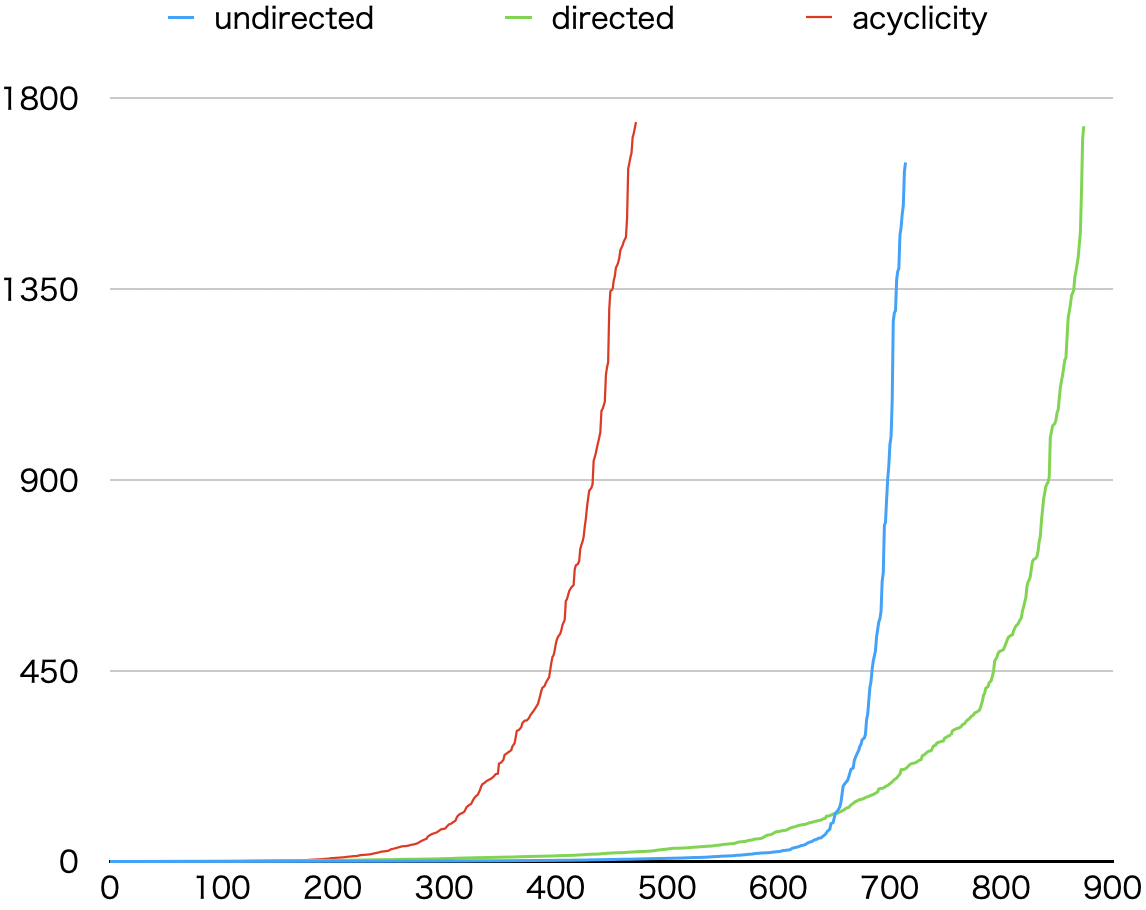
\includegraphics[width=0.8\linewidth]{fig/cactus_fhcp.png}
\caption{ハミルトン閉路問題: カクタスプロット}
\label{cactus}
\end{center}
\end{figure}
%%%%%%%%%%%%%%%%%%%%%%%%%%%%%%%%%%%%%%%%%%%%%%%


%--
本節では,ハミルトン閉路問題の実験結果について述べる.
{\clingo}のオプションは\textit{trendy}を使用し,一問あたりの時間制限を30分とした.
ベンチマーク問題は,\textsf{fhcp}の1001問である.

%--
表~\ref{sat_table}に,各符号化で解けた問題数を,問題の頂点数毎に示す.
左から,問題の頂点数,問題数,各符号化で解けた問題数を示している.
%
解けた問題数は,
\textsf{undirected}符号化が715問,
\textsf{directed}符号化が875問,
\textsf{acyclicity}符号化が473問であり,
\textsf{directed}がもっとも多くの問題を解いた.
\textsf{directed}は,どの頂点数においても同様に,
安定した性能の良さを示した.
図~\ref{cactus}に,カクタスプロットを示す.
縦軸は問題を解くのに要した CPU 時間,横軸は解けた問題数を表す.
グラフが右によるほど多くの問題を解けたことを示し,
下によるほどより速く解けたことを示す.
図~\ref{cactus}より,\textsf{directed}符号化が,
他の2つの符号化と比較して,より多くの問題を高速に解いていることが確認できた.
%% しかし,一部\textsf{undirected}符号化が\textsf{directed}符号化を下回る
%% 部分が確認できる.
%% 実際に,一部の問題では\textsf{undirected}符号化が
%% \textsf{directed}符号化よりも高速に解いていた.

%%%%%%%%%%%%%%%%%%%%%%%%%%%%%%%%%%%%%%%%%%%%%%%%%%%%%%%%%%
\subsection{最短ハミルトン閉路問題}
%%%%%%%%%%%%%%%%%%%%%%%%%%%%%%%%%%%%%%%%%%%%%%%%%%%%%%%%%%

%%%%%%%%%%%%%%%%%%%%%%%%%%%%%%%%%%%%%%%%%%%%%%%
\begin{table}[htbp]
  \caption{実験結果2-1:trendy}
  \label{min_table_tr}
  \centering
  \begin{tabular}{|l|rrr|}
    \hline
    Instance&undirected&directed&acyclicity \\
    \hline
    grid5&50,656*&50,656*&50,656* \\
    grid6&68,656*&68,656*&68,656* \\
    grid7&91,822*&91,822*&91,822* \\
grid8&113,250&\textcolor{red}{112,916}&113,277 \\
grid9&\textcolor{red}{142,502}&143,326&143,660 \\
grid10rc&\textcolor{red}{172,703}&174,866&175,999 \\
grid11&\textcolor{red}{200,399}&204,456&200,638 \\
grid12&\textcolor{red}{231,278}&239,275&232,012 \\
grid13&\textcolor{red}{276,692}&276,926&276,899 \\
grid14&317,617&\textcolor{red}{317,144}&317,676 \\
grid15&\textcolor{red}{375,906}&376,809&376,210 \\
grid16&421,249&\textcolor{red}{419,737}&423,753 \\
US48&11,698*&11,698*&11,698* \\
    \hline
  \end{tabular}
\end{table}
%\label{min_table_tr}
%%%%%%%%%%%%%%%%%%%%%%%%%%%%%%%%%%%%%%%%%%%%%%%

%--
本節では,最短ハミルトン閉路問題の実験結果について述べる.
{\clingo}のオプションは\textit{trendy}を使用し,
一問あたりの時間制限を3時間とした.
ベンチマーク問題は,\textsf{grid}と\textsf{usmap}の合計13問である.

%--
表\ref{min_table_tr}に,各符号化で得られた最適値と最良値を示す.
各問題毎に,最も良かった値を赤字で示している.
*マークは,最適値を表している.
最適値と最良値の数は,
\textsf{undirected}符号化が10問,
\textsf{directed}符号化が7問,
\textsf{acyclicity}符号化が4問であり,
\textsf{undirected}符号化の優位性が確認できた.

%%%%%%%%%%%%%%%%%%%%%%%%%%%%%%%%%%%%%%%%%%%%%%%%%%%%%%%%%%
\subsection{コスト制約付きハミルトン路問題}
%%%%%%%%%%%%%%%%%%%%%%%%%%%%%%%%%%%%%%%%%%%%%%%%%%%%%%%%%%

%%%%%%%%%%%%%%%%%%%%%%%%%%%%%%%%%%%%%%%%%%%%%%%
\begin{table*}[tb]\footnotesize
  \tabcolsep = 2mm
  %\renewcommand{\arraystretch}{1.0}
  \vskip .5em
  \centering
  \begin{tabular}{lr|rrr}
    \hline
    閾値(倍率)    &	解の総数 & \textsf{undirected} & \textsf{directed} & \textsf{acyclicity} \\
    \hline
    11698(1.00)   &	1      &\textbf{2.979} & 7.531 & 4.586	\\
    11814(1.01)   &	8      &5.587  & 15.322	& \textbf{5.250}	\\
    11931(1.02)   &	28     &\textbf{3.243}& 18.600	& 3.578	\\
    12282(1.05)   &	388    &10.003&19.818	& \textbf{6.296}	\\
    12867(1.10)   &	16,180  &16.548& 28.555	& \textbf{9.764}\\
    14037(1.20)   &	939,209 &48.262       &40.717	& \textbf{26.837}\\
    15207(1.30)   &	4,525,541&88.172      &55.276	& \textbf{42.037}\\
    16377(1.40)   &	6,702,964&99.154       &47.647	& \textbf{40.640}	\\
    17547(1.50)   &	6,876,526&95.390       &45.265	& \textbf{38.411}	\\
    18716(1.60)   &	6,876,928&98.937       &49.138	& \textbf{40.748}	\\
    \hline
    平均CPU時間 &   & 46.8275 & 32.7869  & \textbf{21.8147}\\\hline
%    Best    &   & 2 & 0 & \textbf{8} \\ \hline
  \end{tabular}
  \vskip .5em
  \caption{コスト制約付きハミルトン路問題: 解の全列挙に要した CPU 時間}
  \label{cost_table}
\end{table*}
%\label{cost_table}
%%%%%%%%%%%%%%%%%%%%%%%%%%%%%%%%%%%%%%%%%%%%%%%

%--
本節では,第~\ref{chap:background}章でも説明した
コスト制約付きハミルトン路問題(全列挙)の実験結果について述べる.
{\clingo}のオプションは\textit{crafty}を使用し,
一問あたりの時間制限を3時間とした.
ベンチマーク問題は,D.~E~.Knuth の教科書
The Art of Computer Programming~\cite{Knuth:TAOCP:SAT}
に記載されているグラフを使用した(図~\ref{fig:USmap}参照).
このグラフは,米国本土48州の隣接関係を表しており,
頂点数は48,辺の数は105である.
この問題の最短距離は 11698 である(表~\ref{min_table_tr}参照).
今回の実験では,
コスト制約を最短距離のN倍以下
($N=1.00,1.01,1.02,1.05,1.1,1.2,1.3,1.4,1.5,1.6$)として,解の全列挙を
行った.

%--
表~\ref{cost_table}に,各符号化が解の全列挙に要した CPU 時間を示す.
表の1列目はコスト制約の閾値と最短距離からの倍率,2列目は解の総数を表している.
各閾値毎に,最も良かった値を赤字で示している.
表より,
\textsf{acyclicity}符号化が,他の符号化と比較して,より多くの問題を
高速に解いていることがわかる.また,平均CPU時間も最も短い.
%%%%%%%%%%%%%%%%%%%%%%%%%%%%%%%%%%%%%%%%%%%%%%%%%%%%%%%%%%

%%% Local Variables:
%%% mode: latex
%%% TeX-master: "paper"
%%% End:

\chapter{おわりに}\label{chap:conc}

本論文では,電気制約として電流制約のみを考慮した配電網問題および配電網
遷移問題に対して,解集合プログラミング(ASP)を用いた解法を提案した.
配電網(遷移)問題に対する ASP を用いた研究は,著者らの知る限り,本論文
がはじめてである.
提案解法の特長と本論文の貢献について,以下にまとめる.

\begin{description}
\item[表現力:]
  配電網問題を解くための ASP 符号化を考案した.
  ASP 言語の高い表現力を生かし,
  配電網問題の制約を簡潔に記述できることを確認した.
  特に,有向符号化は,無向グラフの各辺$u-v$に対して,2つの弧
  $u\rightarrow v$と$v\rightarrow u$を対応させることで有向グラフ化して
  解く符号化であり,非閉路制約を簡潔に表現できる点が特長である.
\item[拡張性:]
  配電網遷移問題に対して,マルチショット ASP 解法を利用した符号化を提案した.
  この符号化は,配電網問題の ASP 符号化の自然な拡張となっている.
  マルチショット ASP 解法を利用することにより,
  ASP システムが同様の探索失敗を避けるために獲得した学習節を
  (部分的に)保持することで,無駄な探索を避けることができる点が特長である.
\item[効率性:]
  DNET (Power Distribution Network Evaluation Tool)
  に公開されている配電網問題(全3問)と,
  Graph Coloring and its Generalizations
  に公開されているグラフを基に独自に生成したトポロジ制約のみの配電網問
  題(計82問)を用いて実行実験を行なった.
  その結果,有向符号化は,他の2つの符号化と比較して,より多くの問題を
  より高速に解くことができ,その優位性を確認できた.
  %
  配電網遷移問題については,実用規模の問題({\sf fukui-tepco})に対して,
  実行可能解のペアをランダムに選び,合計 1000 問の配電網遷移問題を生成
  し,実行実験を行なった.その結果,すべての問題の到達可能性を判定する
  ことができ,得られた最短ステップ長の最大値は7であった.また,
  マルチショットASP解法を導入することにより,
  通常の解法と比較して,平均で3.8倍の高速化を実現した.
\end{description}

今後の課題としては,電流制約と電圧制約を含む完全な配電網問題への拡張が
挙げられる.しかし,完全な問題は非線形な制約を含むため,標準的な ASP
言語では記述できない.この問題を解決するために,近年研究開発が進められ
ている背景理論付き ASP (ASP Modulo Theories~\cite{DBLP:conf/iclp/GebserKKOSW16}) 
を用いた解法の実現可能性について調査を進める.

%%% Local Variables:
%%% mode: japanese-latex
%%% TeX-master: "paper"
%%% End:

% ここまで

\bibliographystyle{jplain} % 参考文献スタイル
%\bibliography{master,procs,local,lit,akku,aisat}    % 参考文献リスト
\bibliography{procs,local,lit,akku,aisat}    % 参考文献リスト

%%%%%%%%%%%%%%%%%%%%%%%%%%%%%%%%%%%%%%%%%%%%%%%%%%%%%%%%%% 
\chapter*{謝辞}
%%%%%%%%%%%%%%%%%%%%%%%%%%%%%%%%%%%%%%%%%%%%%%%%%%%%%%%%%%

本研究を行うにあたり,
研究の着想から論文執筆にわたり
熱心なご指導を頂いた名古屋大学の番原 睦則教授
に深く感謝申し上げます.
また,本研究だけではなく,様々な相談に乗っていただいた
番原研究室の皆様に感謝申し上げます.
最後に,大学生活を通して支えていただいた家族,友人に
感謝申し上げます.


%%% Local Variables:
%%% mode: japanese-latex
%%% TeX-master: "paper"
%%% End:         % 謝辞

\end{document}
%%%%%%%%%%%%%%%%%%%%%%%%%%%%%%%%%%%%%%%%%%%%%%%%%%%%%%%%%%

%%% Local Variables:
%%% mode: japanese-latex
%%% TeX-master: t
%%% End:
